\documentclass[12pt]{article}
\setlength\headheight{14.5pt}
\title{Exam}
\author{Frederick Robinson}
\date{7 December 2009}
\usepackage{amsfonts}
\usepackage{amsthm}
\usepackage{amsmath}
\usepackage{fancyhdr}
\usepackage{graphicx}
\pagestyle{fancyplain}

\lhead{Frederick Robinson}
\rhead{Math 381: Fourier Analysis}

\begin{document}



   \maketitle

\setcounter{tocdepth}{1} 

\tableofcontents

\section{Problem 1}
\subsection{Question}
Find the steady-state solution of the heat equation on the 3-dimensional shell
\[S=\left\{ x=(x_1,x_2,x_3)\in\mathbb{R}^3:R_1\leq |x| \leq R_2 \right\}\]
with the inner temperature $u=T_1$ and outer temperature $u=T_2$.

\subsection{Answer}\label{1::}
The heat equation is $u_t = K \nabla ^2 u$  and since the problem has spherical symmetry we will employ spherical coordinates. We know that \cite[Page 237]{pinsky} the Laplacian is given in spherical coordinates by
\[\nabla^2 u = u_{rr} +\frac{2}{r} u_r+ \frac{1}{r^2} \left( u_{\theta \theta} +\cot{\theta} u_\theta  +  \csc^2{\theta} u_{\varphi \varphi} \right)\]

With in this mind we now se that steady state solutions to the heat equation in the given shell will satisfy 
\[0=u_t=K \nabla^2 u = K \left( u_{rr} +\frac{2}{r} u_r+ \frac{1}{r^2} \left( u_{\theta \theta} +\cot{\theta} u_\theta  +  \csc^2{\theta} u_{\varphi \varphi} \right) \right) \]
and since the boundary conditions are radially symmetric we observe further that 
\[0=  u_{rr} +\frac{2}{r} u_r \]

Now we need only solve the above ordinary differential equation which we can do as follows. 
\[  \text{Let } v=u_r \Rightarrow v_r=u_{rr}\]
So
\[0=  u_{rr} +\frac{2}{r} u_r \Leftrightarrow 0= v_r +\frac{2}{r} v\]
now
\begin{eqnarray*}0 &=& v_r +\frac{2}{r} v\\
-\frac{2}{r} v &=& \frac{d v}{d r} \\
-\frac{2}{r} dr &=& \frac{1}{v} dv \\
\end{eqnarray*}
Integrating we get
\begin{eqnarray*}
-\frac{2}{r} dr &=& \frac{1}{v} dv \\
- 2\int \frac{1}{r} dr &=& \int \frac{1}{v} dv \\
\end{eqnarray*}
so
\[-2 \ln{r} = \ln{v} +C\]
for some arbitrary constant $C$.
\[\Rightarrow v(r) = \frac{e^C}{r^2} \]
For convenience we will rename constants yielding
\[\Rightarrow v(r) = \frac{C}{r^2} \]
Now it remains only to translate this to a statement about $u$. From our definition of $v$ we can do this as follows
\[   v=u_r = \frac{d u}{d r}\]
so we have in particular 
\begin{eqnarray*}
\frac{d u}{d r} &=& \frac{C}{r^2} \\
 \Rightarrow \frac{1}{C} du &=& \frac{1}{r^2} dr
\end{eqnarray*}
again integration yields
\begin{eqnarray*}
\frac{1}{C}  \int du &=&  \int \frac{1}{r^2} dr \\
\frac{u}{C} &=&  - \frac{1}{r} +K  \\
u &=&C \left(  - \frac{1}{r} +K  \right) \\
\end{eqnarray*}
for some arbitrary choice of $K$. We can further rename our constants to get the solution as
\begin{equation}\label{1:gensol}u(r) =  K - \frac{C}{r} \end{equation}

Now that we have computed the general form of the radially symmetric steady state solution to the heat equation in a spherical shell it remains only to apply our boundary conditions. These are: $u(R_1)=T_1$ and $u(R_2)=T_2$.

Applying our boundary conditions we get 
\begin{equation}\label{1:eq1}u(R_1)=T_1= K - \frac{C}{R_1} \end{equation}
and
\begin{equation}\label{1:eq2}u(R_2)=T_2= K - \frac{C}{R_2} \end{equation}
so subtracting yields
\begin{eqnarray*}
T_1 - T_2  &=& \frac{C}{R_2} - \frac{C}{R_1}  \\
T_1 - T_2  &=& \frac{C (R_1 - R_2)}{R_1 R_2}  \\
C &=& \left(T_1 - T_2 \right) \left( \frac{ R_1 R_2}{R_1 - R_2} \right)  \\
\end{eqnarray*}

Now it is easy to recover the value of $K$. We just use Equation \ref{1:eq1} together with our newly acquired value for $C$.
\begin{eqnarray*}
T_1 &=&  K - \frac{C}{R_1} \\
 T_1 &=&  K - \frac{1}{R_1} \left(T_1 - T_2 \right) \left( \frac{ R_1 R_2}{R_1 - R_2} \right)   \\
 K &=&  T_1 + \frac{1}{R_1} \left(T_1 - T_2 \right) \left( \frac{ R_1 R_2}{R_1 - R_2} \right)   \\
   &=&  T_1 + \left(T_1 - T_2 \right) \left( \frac{R_2}{R_1 - R_2} \right)   \\
    &=& \frac{T_1 (R_1-R_2)}{R_1-R_2}+ \left( \frac{R_2 \left(T_1 - T_2 \right) }{R_1 - R_2} \right)   \\
        &=& \frac{T_1 (R_1-R_2)+R_2 \left(T_1 - T_2 \right) }{R_1 - R_2}  \\
   &=& \frac{T_1 R_1-T_1 R_2+R_2  T_1 -  R_2 T_2  }{R_1 - R_2}  \\
   &=& \frac{T_1 R_1 - T_2   R_2 }{R_1 - R_2}  \\
\end{eqnarray*}

Combining these values for our constant with the general solution (\ref{1:gensol}) we get
\begin{eqnarray*}
u(r) &=&   \frac{T_1 R_1 - T_2   R_2 }{R_1 - R_2}   - \left( \frac{1}{r} \right) \left( \left(T_1 - T_2 \right) \left( \frac{ R_1 R_2}{R_1 - R_2} \right)  \right) \\
&=&  \frac{1}{R_1 - R_2}  \left(  \left( T_1 R_1 - T_2   R_2 \right)   - \left( \frac{ R_1 R_2 }{r} \right)  \left(T_1 - T_2 \right)  \right) \\
\end{eqnarray*}

We can check that in the case that the inner temperature and the outer temperature are the same the steady state solution is that in which the entire shell has this same temperature. That is, if $T-1=T_2=T$ then
\begin{eqnarray*}
u(r) &=&  \frac{1}{R_1 - R_2}  \left(  \left( T_1 R_1 - T_2   R_2 \right)   - \left( \frac{ R_1 R_2 }{r} \right)  \left(T_1 - T_2 \right)  \right) \\
&=&  \frac{1}{R_1 - R_2}    \left( T R_1 - T   R_2 \right) \\
&=&  T\\
\end{eqnarray*}
as we would expect

\subsubsection{Figures}
Plots of temperature versus radius for $R_1=1$ and $R_2=2$ for various inner and outer temperatures.

\begin{figure}[htp]
\centering
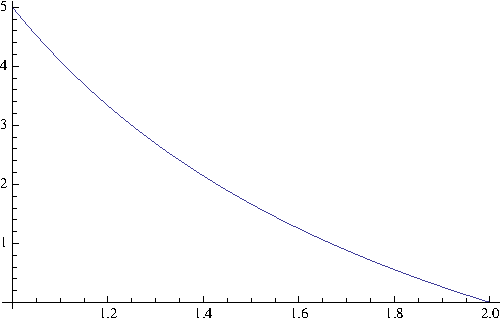
\includegraphics{5to0.pdf}
\caption{Inner temperature $T_1=5$ with outer temperature $T_2=0$}\label{fig:5to0}
\end{figure}

\begin{figure}[htp]
\centering
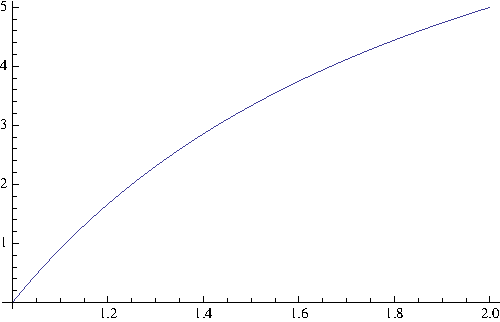
\includegraphics{0to5.pdf}
\caption{Inner temperature $T_1=0$ with outer temperature $T_2=5$}\label{fig:0to5}
\end{figure}

\begin{figure}[htp]
\centering
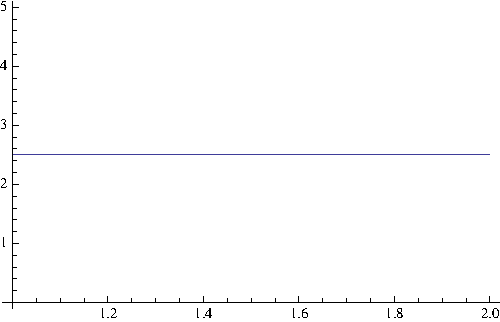
\includegraphics{flat.pdf}
\caption{Inner temperature $T_1=2.5$ with outer temperature $T_2=2.5$}\label{fig:flat}
\end{figure}

\section{Problem 2}
\subsection{Question}
Calculate the solutions of separated variables of the heat equation in the interval $[0,L]$ that satisfy the boundary conditions
\[u(0;t)=u_x(L;t)=0.\]

\subsection{Answer}
We are seeking separated solutions to this problem, which means in particular that we are looking for a function of the form $u(x;t)=X(x)T(t)$ that satisfies the heat equation $u_t = K u_{xx}$

So, applying the heat equation to the form of the solution and employing the product rule we see that 
\[XT'=KX''T\]
\[\frac{T'}{KT}=\frac{X''}{X}\]
Since the left side of this equation depends only on time and the right side depends only on position we may surmise that they are both constant valued. So, 
\[\frac{T'}{KT}=\frac{X''}{X}=-\lambda\]

Now we have reduced the problem to the pair of ordinary differential equations
\begin{equation}\label{2:t} T'+\lambda K T = 0 \end{equation}
\begin{equation}\label{2:x} X''+\lambda X = 0 \end{equation}

Equation \ref{2:t} has solution 
\[T(t)=e^{-\lambda K t}\]
which is never zero. To obtain the function $X(x)$ we must employ the boundary conditions.
\[u(0;t)=u_x(L;t)=0\]
Now however we see that this is just a Sturm-Liouville eigenvalue problem. That is, the separated solutions of the given heat equation are 
\[u(x;t)=e^{-\lambda_n K t}X_N(x)\] 
where $\lambda_n$ is an eigenvalue and $X_n$ is an eigenfunction of the Sturm-Liouville eigenvalue problem  $X''(x)+\lambda X(x) = 0$. 

But we know from \cite[Exercise 1 Page 96]{pinsky} (see also Appendix \ref{slproblem}) that the solution to this Sturm-Liouville eigenvalue problem is 
\[X_n= A \sin{\frac{\pi x(n-\frac{1}{2})}{L}} \quad \lambda_n=\left( \frac{\pi (n-\frac{1}{2})}{L} \right)^2 \quad n=1,2,\dots \]
Thus we may conclude finally that the separated solutions for the heat equation in the interval $[0,L]$ that satisfy the boundary conditions $u(0;t)=u_x(L;t)=0$ are
\[u(x;t)=A e^{- \left( \frac{\pi (n-\frac{1}{2})}{L} \right)^2 \ K t} \sin{\frac{\pi x(n-\frac{1}{2})}{L}} \] 
for some arbitrary constant $A$ and $n \in \mathbb{N}$.


\section{Problem 3}
\subsection{Question}
Compute the Fourier coefficients of the function $f(x)=x^3$ on the interval $[-L,L]$ and describe the values of the Fourier series at all points $x\in(-\infty,\infty)$.

\subsection{Answer}

The fourier coefficients of a real-valued function $f(x)$, $-L<x<L$ are given by \cite[Page 37]{pinsky} as
\[A_0 = \frac{1}{2 L} \int_{-L}^L f(x) dx \]
\[A_n = \frac{1}{L} \int_{-L}^L f(x) \cos{\frac{n \pi x}{L}} dx \quad  n=1,2,\dots\]
\[B_n = \frac{1}{L} \int_{-L}^L f(x) \sin{\frac{n \pi x}{L}} dx \quad n=1,2,\dots \]

Now we just use these definitions to compute the Fourier coefficients.

We begin by computing $A_0$
\begin{eqnarray*}A_0 &=& \frac{1}{2 L} \int_{-L}^L x^3 dx \\
&=& \frac{1}{2L} \left[\frac{x^4}{4}\right]_{-L}^L \\
&=& \frac{1}{2L} \left(\frac{L^4}{4}-\frac{(-L)^4}{4}\right)\\
&=& \frac{1}{2L} \left(\frac{L^4}{4}-\frac{L^4}{4}\right)\\
&=& 0
\end{eqnarray*}

Then we compute $A_n$ by
\[A_n = \frac{1}{L} \int_{-L}^L x^3 \cos{\frac{n \pi x}{L}} dx 
\]
but there is no need to explicitly compute this integral since we observe that $x^3$ is an odd function and $\cos{\frac{n \pi x}{L}}$ is an even one. Since the product of an odd and an even function is an odd function and we are taking the integral over the interval $-L, L$ the integral is just zero. For, the integral from $-L$ to $0$ is precisely $-1$ times the integral from $0$ to $L$. 

\[A_n=0\]

We can also arrive at this conclusion by observing that by definition of Fourier sine series \cite[Page 42]{pinsky} the fact that $f(x)=x^3$ is odd means that our fourier series is only in terms of its sine coefficients $B_n$.

So now we compute these sine coefficients by 
\[B_n = \frac{1}{L} \int_{-L}^L x^3 \sin{\frac{n \pi x}{L}} dx\\
\]
however we observe that since both $x^3$ and $\sin{\frac{n \pi x}{L}}$ are odd functions their product is an even one. Hence, we need only integrate over half of $(-L,L)$ then multiply the resulting quantity by $2$.
\begin{eqnarray*}B_n &=& \frac{2}{L} \int_{0}^L x^3 \sin{\frac{n \pi x}{L}} dx\\
&=& \frac{2}{L} \int_{0}^L x^3 \sin{\frac{n \pi x}{L}} dx\\
\end{eqnarray*}
Now we must integrate by parts. Recall that
\[\int_a^b u dv = \left[u v \right]_a^b - \int_a^b v du\]
In particular we shall let
\[u=x^3 \quad dv=\sin{\frac{n \pi x}{L}}\]
\[du=3 x^2 \quad v= -\frac{L}{n \pi} \cos{\frac{n \pi x}{L}}\]
so we see that
\begin{eqnarray*}B_n &=& \frac{2 }{L} \left( \left[-\frac{x^3 L}{n \pi} \cos{\frac{n \pi x}{L}}  \right]_{0}^L + \frac{3 L}{n \pi} \int_{0}^L   \cos{\frac{n \pi x}{L}}  x^2  \right) \\
&=& \frac{2 }{L} \left( -\frac{L^4 }{n \pi} (-1)^n   + \frac{3 L}{n \pi} \int_{0}^L   \cos{\frac{n \pi x}{L}}  x^2  \right) \\
&=&   \frac{2 L^3 (-1)^{n+1} }{n \pi}    + \frac{6 }{n \pi} \int_{0}^L   \cos{\frac{n \pi x}{L}}  x^2 \\
\end{eqnarray*}
We must again integrate by parts. Let
\[u=x^2 \quad \ dv=\cos{\frac{n \pi x }{L}}\]
\[du=2x \quad v= \frac{L}{n \pi } \sin{\frac{n \pi x}{L}}\]
to get 
\begin{eqnarray*}B_n &=&  \frac{2 L^3 (-1)^{n+1} }{n \pi}    + \frac{6 }{n \pi} \left( \left[ \frac{L x^2}{n \pi} \sin{\frac{n \pi x}{L}} \right]_0^L - 2 \int_0^L \frac{xL}{n\pi} \sin{\frac{n \pi x}{L}} \right) \\
&=&  \frac{2 L^3 (-1)^{n+1} }{n \pi}    + \frac{-12 }{n \pi}  \int_0^L \frac{xL}{n\pi} \sin{\frac{n \pi x}{L}}   \\
&=&  \frac{2 L^3 (-1)^{n+1} }{n \pi}    + \frac{-12 L}{(n \pi)^2}  \int_0^L x \sin{\frac{n \pi x}{L}}   \\
\end{eqnarray*}
Finally we apply integration by parts one last time, now with
\[u=x \quad dv = \sin{\frac{n \pi x}{L}} \]
\[ du = 1 \quad v = - \frac{L}{n \pi } \cos{\frac{n \pi x}{L}} \]
arriving at 
\begin{eqnarray*}B_n &=&  \frac{2 L^3 (-1)^{n+1} }{n \pi}    + \frac{-12 L}{(n \pi)^2}  \left( \left[ - \frac{x L}{n \pi } \cos{\frac{n \pi x}{L}}   \right]_0^L + \frac{L}{n \pi } \int_0^L  \cos{\frac{n \pi x}{L}} \right)  \\
 &=&  \frac{2 L^3 (-1)^{n+1} }{n \pi}    + \frac{-12 L}{(n \pi)^2}  \left(  - \frac{ L^2 }{n \pi } \cos{n \pi }   + \frac{L}{n \pi } \int_0^L  \cos{\frac{n \pi x}{L}} \right)  \\
  &=&  \frac{2 L^3 (-1)^{n+1} }{n \pi}    +   \frac{12 L^3}{(n \pi)^3}   \cos{n \pi }   +  \frac{-12 L^2}{(n \pi)^3}  \int_0^L  \cos{\frac{n \pi x}{L}}   \\
  &=&  \frac{2 L^3 (-1)^{n+1} }{n \pi}    +   \frac{12 L^3}{(n \pi)^3}   (-1)^n   +  \frac{-12 L^3}{(n \pi)^4}  \left[ \sin{\frac{n \pi x}{L}}  \right]_0^L \\
  &=&  \frac{2 L^3 (-1)^{n+1} }{n \pi}    +   \frac{12 L^3}{(n \pi)^3}   (-1)^n  \\
    &=& \frac{ 2 L^3}{n \pi}\left(    \frac{6}{(n \pi)^2}  -1 \right)  (-1)^n  \\
\end{eqnarray*}

So all together we have 
\begin{eqnarray*}A_0 &=& 0 \\
A_n &=& 0 \\
B_n  &=& \frac{ 2 L^3}{n \pi}\left(    \frac{6}{(n \pi)^2}  -1 \right)  (-1)^n  \\
\end{eqnarray*}

Thus the Fourier series for the function $f(x)=x^3$ is given by
\[ \sum_{n=1}^\infty \frac{ 2 L^3}{n \pi}\left(    \frac{6}{(n \pi)^2}  -1 \right)  (-1)^n  \sin{\frac{n \pi x}{L}} \]

By \cite[Theorem 1.1 Page 49]{pinsky} we know that the Fourier series will converge to$ \frac{1}{2}\left[ \bar{f} (x+0) + \bar{f} (x-0) \right]$ (where$\bar{f}$ is the 2L-periodic extension of $f(x)$ limited to $-L < x< L$) since $f$ is piecewise smooth. So, in particular we know that the Fourier series will converge to 
\[g(x)= \left\{
\begin{array}{lr}
y^3 & y \in (-L,L) \quad y = x-2nL \quad x \neq n L\\
0 & x=n L
\end{array} \right.  \quad n\in \mathbb{Z}\]
where $g(x)$ is the Fourier series for $f$ on the interval $(-L,L)$. That is, it converges to the 2-L periodic extension of $f$ except on the points between these extensions where it converges to the arithmetic mean of the value on either end: $\frac{1}{2}((-L)^3+L^3)=0$.

\subsubsection{Figures}
\begin{figure}[htp]
\centering
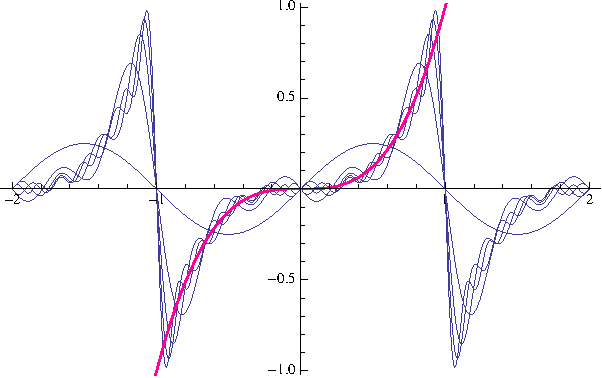
\includegraphics{fourierseriesfigure.pdf}
\caption{Some early terms of the fourier series, along with $x^3$ ($L=1$)}\label{fig:fsf}
\end{figure}


\section{Problem 4}
\subsection{Question}
Choose an appropriate function to expand into its Fourier series and use Parseval's theorem to evaluate the sum
\[\zeta(4)=\sum_{n=1}^\infty \frac{1}{n^4}.\]

\subsection{Answer}
We shall expand the function
\[f(x) = x^2 \quad x\in[-\pi,\pi]\]
to a Fourier series and compute its mean square error.

We begin by observing that $f(x) = x^2$ is an even function. So we know that the Fourier series corresponding to $f$ must be a Fourier cosine series. That is
\[f(x)=A_0+ \sum_{n=1}^\infty A_n \cos{n x}\]
where the $A_n$ are the Fourier coefficients for cosine and given by
\[A_n=\frac{2}{\pi}\int_{0}^\pi x^2 \cos{nx} dx\]
Setting
\[u=x^2 \quad dv = \cos{nx} \]
\[du=2x \quad v = \frac{1}{n} \sin{nx} \]
and integrating by parts we get
\begin{eqnarray*}
A_n &=& \frac{2}{\pi}\left( \left[ \frac{x^2}{n}\sin{nx}\right]_0^\pi  - \frac{2}{n} \int_{0}^\pi x \sin{nx} \right)\\
&=&    - \frac{4}{\pi n} \int_{0}^\pi x \sin{nx} \\
\end{eqnarray*}
Now we let
\[u=x \quad dv = \sin{nx} \]
\[du=1 \quad v = -\frac{1}{n} \cos{nx} \]
and again integrate by parts yielding
\begin{eqnarray*}
A_n &=&  - \frac{4}{\pi n} \left( - \left[\frac{x}{n}\cos{n x} \right]_0^\pi + \int_0^\pi \frac{1}{n} \cos{n x} \right)\\
 &=&  - \frac{4}{\pi n} \left( - \frac{\pi}{n} \left((-1)^n  \right) + \int_0^\pi \frac{1}{n} \cos{n x} \right)\\
 &=&  - \frac{4}{\pi n} \left( - \frac{\pi}{n} \left((-1)^n  \right) + \frac{1}{n^2} \left[  \sin{n x} \right]_0^\pi \right) \\
 &=&   \frac{4 \pi}{n^2 \pi} \left((-1)^n  \right)  \\
 &=&   \frac{4 }{n^2 } (-1)^n   \\
\end{eqnarray*}

Now we just compute $A_0$ by
\[\frac{1}{\pi}A_0=\int_{-\pi}^\pi x^2 dx \]
\[A_0=\frac{2 \pi ^2}{3}\]

So 
\[f(x)= \frac{2 \pi ^3}{3} + \sum_{n=1}^\infty  \frac{4 }{n^2 } (-1)^n  \cos{n x}\]

Now we may compute the mean squared error by \cite[Page 72]{pinsky}
\begin{eqnarray*}
\sigma^2_N &=& \frac{1}{2} \sum_{n=N+1}^\infty (A_n^2+B_n^2)\\
 &=& \frac{1}{2} \sum_{n=N+1}^\infty \left(\frac{4 }{n^2 } (-1)^n \right)^2\\
 &=& \frac{1}{2} \sum_{n=N+1}^\infty \frac{16 }{n^4 } \\
 &=& 8\sum_{n=N+1}^\infty \frac{1 }{n^4 } \\
\end{eqnarray*}

But now we are in a position to employ Parseval's Theorem which states \cite[Page 71]{pinsky}\footnote{Actually, this is not the definition of Parseval's theorem that appears in Pinsky. However after many unsuccessful tries with his definition I looked on the internet \cite{parseval} and found this definition.}
\[\frac{1}{2 L} \int_{-L}^L f(x)^2 dx = \frac{A_0^2}{4}+\frac{1}{2} \sum_{n=1}^\infty (A_n^2 +B_m^2)\]
or equivalently
\[\frac{1}{2 L} \int_{-L}^L f(x)^2 dx = \frac{A_0^2}{4}+\sigma_0^2\]

In this case we have
\[\frac{1}{2\pi} \int_{-\pi}^\pi (x^2)^2 dx = \left(\frac{2 \pi ^2}{3}\right)^2\frac{1}{4}+ 8\sum_{n=1}^\infty \frac{1 }{n^4 } \]
\[\frac{1}{10 \pi} \left[  x^5 \right]_{-\pi}^\pi= \left(\frac{2 \pi ^2}{3}\right)^2\frac{1}{4}+ 8\sum_{n=1}^\infty \frac{1 }{n^4 } \]
\[\frac{1}{10 \pi} \left(  \pi^5 + \pi^5 \right)=  \left(\frac{2 \pi ^2}{3}\right)^2\frac{1}{4}+ 8\sum_{n=1}^\infty \frac{1 }{n^4 } \]
\[\frac{2 \pi^5}{10 \pi} = \left(\frac{2 \pi ^2}{3}\right)^2\frac{1}{4} + 8\sum_{n=1}^\infty \frac{1 }{n^4 } \]
\[\frac{2 \pi^5}{10 \pi} = \frac{\pi ^4}{9} + 8\sum_{n=1}^\infty \frac{1 }{n^4 } \]
\[ \frac{1}{8} \left( \frac{2 \pi^5}{10 \pi} - \frac{\pi ^4}{9} \right)=   \sum_{n=1}^\infty \frac{1 }{n^4 } \]
\[ \frac{1}{8} \left(\frac{4 \pi ^4}{45} \right)=   \sum_{n=1}^\infty \frac{1 }{n^4 } \]
\[ \frac{ \pi ^4}{90} =   \sum_{n=1}^\infty \frac{1 }{n^4 } \]

and so the $\zeta(4)= \frac{ \pi ^4}{90}$ for $\zeta$ the Riemann zeta function. 


\section{Problem 5}
\subsection{Question}
Show that if there is a steady-state solution of the non-homogeneous solution to the equation $u_t=K\Delta u +r$ in the slab $\{(x,y,z) : 0\leq z \leq L \} \subset \mathbb{R}^3$ satisfying the boundary conditions
\[u_z(x,y,0;t)=C_1, u_z(x,y,L;t)=C_2, \]
then $K(C_2-C_1)+r L = 0$, What is the physical interpretation of this relation?

\subsection{Answer}
Since the boundary conditions are independent of both $x$ and $y$ we must only have solutions of the form $U(z)$. So in particular we have
\[K U''(z)+r=0\]
and we know that the general solution to this ordinary differential equation is
\[U(z)=\frac{-r z^2}{2 K}+A+B z\]
Now we just apply the boundary conditions.
\begin{eqnarray*}
U(z) &=& \frac{-r z^2}{2 K}+A+B z \\
U'(z) &=& \frac{-r z}{ K}+B \\
U'(z) &=& \frac{-r (0)}{ K}+B = C_1 \\
B &=& C_1 \\
\end{eqnarray*}
and
\begin{eqnarray*}
U(z) &=& \frac{-r z^2}{2 K}+A+B z \\
U'(z) &=& \frac{-r z}{ K}+B \\
U'(L) &=& \frac{-r (L)}{ K}+C_1 = C_2 \\
U'(L) &=& \frac{-r (L)}{ K}= C_2 - C_1 \\
\frac{-r (L)}{ K} &=& C_2 - C_1 \\
-r L &=& (C_2 - C_1)K \\
0 &=& r L + K (C_2 - C_1) \\
\end{eqnarray*}
as desired. Physically we can interpret this as meaning if heat is being lost at the edges of a slab with some sort of heat source, the amount of heat being added to the system by this source must be exactly in balance with that being lost at the edges. Otherwise there will not be a steady state solution. What's more we can also say that the only thing that matters (in terms of the magnitude of the corresponding heat source) is the size of the difference between $C_1$ and $C_2$ and the absolute magnitude of $K$ as opposed to the absolute sizes of $C_i$.



\section{Problem 6}
\subsection{Question}
Find the solution of the following initial-boundary value problem of the heat equation
\[u_t=K u_{zz} + v e^{-at} \sin{\frac{\pi z}{L}},  0<z<L, t>0,\]
\[u(0;t)=u(L;t)=0,\]
\[u(z;0)=0. \]

\subsection{Answer}
We recognize that this is just a temporally nonhomogeneous problem heat equation problem whose solution is outlined on \cite[Page 131]{pinsky}. First we have homogeneous boundary conditions: that is $t_1=T_2=0$. Thus, we seek the solution in the form of a series of eigenfunctions of the homogeneous problem.
\[r(z;t)=\sum_{n=1}^\infty r_n(t)\phi_n(z), \quad f(z) = \sum_{n=1}^\infty f_n\phi_n(z), \quad u(z;t)= \sum_{n=1}^\infty u_n(t) \phi_n(z)\]
where $\phi_n(z)$ are normalized eigenfunctions of the Sturm-Liouville eigenvalue problem with the associated boundary conditions. The expansion coefficients $r_n(t)$, $f_n$, and $u_n(t)$ are obtained from the orthogonality of the eigenfunctions as the generalized Fourier coefficients:
\[r_n(t)=\int_0^L r(z;t)\phi_n(z)dz, \quad f_n = \int_0^L f(z) \phi_n(z) dz , \quad u_n(t)= \int_0^L u(z;t) \phi_n(z) dz\]
substituting the series for u(z;t) in the nonhomogeneous heat equation we get
\[u_t-K u_{zz}=\sum_{n=1}^\infty \left[ u'_n(t)+K\lambda_n u_n(t)\right]\phi_n(z) = \sum_{n=1}^\infty r_n(t) \phi_n(z) \]
so we therefore must choose $u_n(t)$ such that it solves the ordinary differential equation 
\[ u'_n(t)+K\lambda_n u_n(t)= r_n(t)\]
with initial conditions $u_n(0)=f_n$. It is easy to see that the solution is of the form
\[u_n(t)=f_n e^{-\lambda_N K t} + \int_0^t r_n(s) e^{-\lambda_n K (t-s)}ds\]
In our case however we have $f=0$ so this reduces further to
\[u_n(t)= \int_0^t r_n(s) e^{-\lambda_n K (t-s)}ds\]


\[u(z;t)=v \sin{\left( \frac{\pi z}{L} \right) }\frac{e^{-a t}-e^{-\pi^2K t / L^2}}{a-(\pi^2 K/L^2)} \quad a\neq \frac{\pi^2 K}{L^2} \]
\[u(z;t)=v \sin{\left( \frac{\pi z}{L} \right) }t e^{-\pi^2K t /L^2} \quad a = \frac{\pi^2 K}{L^2} \]


\section{Problem 7}
\subsection{Question}
Let $u$ be a harmonic function in the plane. Use Poisson's formula to show that the value of the function at the center of a circle is the average value of its values on the circle.

\subsection{Answer}

Since $u$ is a harmonic function we know that it is twice differentiable and satisfies Laplace's equation. That is, $\nabla^2 u = 0$. Moreover we know that we can compute the value of $u$ using the Poisson integral formula \cite[Page 180]{pinsky} 
\[u(\rho , \varphi) = \frac{1}{2 \pi} \int_{-\pi}^\pi \frac{R^2-\rho^2}{R^2-\rho^2-2R\rho\cos{(\psi - \varphi)}} T(\psi)d \psi \quad 0 \leq \rho < R\]

So if we set $\rho=0$ we just get
\[u(0 , \varphi) = \frac{1}{2 \pi} \int_{-\pi}^\pi T(\psi)d \psi \quad 0 \leq \rho < R\]
but this is just the average of $T$ as desired.

Furthermore, since translating a solution of Laplace's equation generates an equation which still satisfies Laplace's equation it follows that we can translate a given solution of Laplace's equation so that any point we wish is at the origin. Then we get the above result for any arbitrary point in a solution to Laplace's equation.


\section{Problem 8}
\subsection{Question}
Find all radially symmetric solutions of the equation $\Delta u = -1$ in $\mathbb{R}^3$.

\subsection{Answer}

We will use the spherical laplacian
\[\nabla^2 u = u_{rr} +\frac{2}{r} u_r+ \frac{1}{r^2} \left( u_{\theta \theta} +\cot{\theta} u_\theta  +  \csc^2{\theta} u_{\varphi \varphi} \right)\]
in this case as it reduces the work significantly. 

Since our solutions must be radially symmetric we must have
\[\nabla^2 u = u_{rr} +\frac{2}{r} u_r \]
\[-1 = u_{rr} +\frac{2}{r} u_r \]
but in Section \ref{1::} we showed that the solution to the homogeneous form of this ordinary differential equation is just
\[u(r)=K-\frac{C}{r}\]
for arbitrary choice of $C$, $K$. Furthermore one can check (see Appendix \ref{check}) that $u=-\frac{1}{6}r^2$ is a particular solution to this differential equation. Hence the general solution can be obtained as a summation of the solution to the homogenous problem and the particular solution. That is
\[u(r)=K-\frac{C}{r}-\frac{1}{6}r^2\]



\section{Problem 9}
\subsection{Question}
Calculate the Fourier transform of the following functions

(a) $f(x) = x e^{-|x|}$;

(b) $f(x) = e^{-x^2 -2x}$;

(c) $f(x) = x^2 e^{-x^2/2}$;

(d) $f(x) = e^{-2 |x|} \sin{x}$.

\subsection{Answer}
\textbf{(a)} \emph{$f(x) = x e^{-|x|}$}

We know that the definition of the Fourier transform is 
\[f(\mu) = \frac{1}{2 \pi} \int_{-\infty}^\infty f(x) e^{-i \mu x} dx\]
so we substitute into this definition to yield
\[f(\mu) = \frac{1}{2 \pi} \int_{-\infty}^\infty  x e^{-|x|} e^{-i \mu x} dx\]
Then split the limits of integration to
\[f(\mu) = \frac{1}{2 \pi} \left( \int_{-\infty}^0  x e^{x} e^{-i \mu x} dx + \int_{0}^\infty  x e^{-x} e^{-i \mu x} dx \right) \]
\[= \frac{1}{2 \pi} \left( \int_{-\infty}^0  x  e^{x(1-i \mu) } dx + \int_{0}^\infty  x  e^{x(-1-i \mu )} dx \right) \]
\[= \frac{1}{2 \pi} \left(\frac{1}{(i+\mu )^2}+\frac{1}{(1+i \mu )^2}\right)\]
\[= \frac{2 \mu}{i \pi (1+\mu^2)^2} \]

\textbf{(b)} \emph{$f(x) = e^{-x^2 -2x}$}

Again let's apply the definition of the Fourier transform
\[f(\mu) = \frac{1}{2 \pi} \int_{-\infty}^\infty f(x) e^{-i \mu x} dx\]
so we substitute into this definition to yield
\[f(\mu) = \frac{1}{2 \pi} \int_{-\infty}^\infty e^{-x^2 -2x} e^{-i \mu x} dx\]
\[= \frac{1}{2 \pi} \int_{-\infty}^\infty e^{-x^2 -2x-i \mu x}  dx\]
\[= \frac{1}{2 \pi} \int_{-\infty}^\infty e^{-x^2 -x(2+i \mu )}  dx\]
Integrating yields
\[\frac{1}{2\pi} e^{-\frac{1}{4} (-2 i+\mu )^2} \sqrt{\pi }\]

\textbf{(c)} \emph{$f(x) = x^2 e^{-x^2/2}$}

Again let's apply the definition of the Fourier transform
\[f(\mu) = \frac{1}{2 \pi} \int_{-\infty}^\infty f(x) e^{-i \mu x} dx\]
so we substitute into this definition to yield
\[f(\mu) = \frac{1}{2 \pi} \int_{-\infty}^\infty x^2 e^{-x^2/2} e^{-i \mu x} dx\]
\[f(\mu) = \frac{1}{2 \pi} \int_{-\infty}^\infty x^2  e^{-i \mu x -x^2/2} dx\]
Integrating we get 
\[-e^{-\frac{u^2}{2}} \left(-1+u^2\right)\]


\textbf{(d)} \emph{$f(x) = e^{-2 |x|} \sin{x}$}
Again let's apply the definition of the Fourier transform
\[f(\mu) = \frac{1}{2 \pi} \int_{-\infty}^\infty f(x) e^{-i \mu x} dx\]
so we substitute into this definition to yield
\[f(\mu) = \frac{1}{2 \pi} \int_{-\infty}^\infty  e^{-2 |x|} \sin{x} e^{-i \mu x} dx\]
\[f(\mu) = \frac{1}{2 \pi} \int_{-\infty}^\infty   \sin{x} e^{-i \mu x-2 |x|} dx\]
and we integrate to get
\[\frac{4 i  \mu }{25+6 \mu ^2+\mu ^4}\]


\section{Problem 10}
\subsection{Question}
Find the solution of the heat equation $u_t=K u_{xx}$ for $t>0$, $x>0$ with the boundary condition $u(0;t) = 0$ and the initial condition $u(x;0) = 1$ for $0\leq x \leq L$ and $u(x;0) = 0$ for $x>L$.

\subsection{Answer}
This is just a Dirichlet boundary condition problem whose solution is given \cite[Page 304]{pinsky} by 
\[u(x;t)=\frac{1}{\sqrt{r \pi K t}}\int_0^\infty e^{-(x-\xi)^2/4 K t}-e^{-(x+\xi)^2/4 K t} f(\xi) d\xi\]

In this case we have 
\[f=\left\{\begin{array}{lr}
1& x \leq L\\
0 & x > L\\
\end{array}\right.\]

So the solution to our problem just becomes 
\[u(x;t)=\frac{1}{\sqrt{r \pi K t}}\int_0^L e^{-(x-\xi)^2/4 K t}-e^{-(x+\xi)^2/4 K t}  d\xi\]


\section{Problem 11}
\subsection{Question}
Consider the heat equation $u_t = K u_{xx} + a u$ in the region $t>0$, $-\infty < x < \infty$ with the initial conditions $u(x;0) = e^{-x^2}$ where $a$ is a positive constant. Express the solution of this problem in terms of the error function
\[\Phi(z) = \frac{1}{\sqrt{2 \pi}} \int_{-\infty}^z e^{-\xi^2 /2} d \xi .\]


\subsection{Answer}

We will first solve this problem in general, for $ u(x;0)=f(x)$

Now we will look for solutions as Fourier series in analogy to the process used to determine the solution to such equations without a source term in 5.2.2 \cite[Page 295]{pinsky}. So, let $U(\mu;t)$ be the Fourier transform of $u(x;t)$. So, from the definition of a Fourier transform we have 
\begin{equation}\label{reverse}u(x;t)=\int_{-\infty}^\infty U(\mu;t) e^{i \mu x}d\mu\end{equation}
and
\begin{equation}\label{forwards}U(\mu;t)=\frac{1}{2\pi}\int_{-\infty}^\infty u(x;t) e^{-i \mu x}dx\end{equation}

Now we shall assume that derivatives can be taken under the integral signs to obtain 
\[u_t(x;t)=\int_{-\infty}^\infty U_t(\mu;t) e^{i \mu x} d\mu\]
\[u_x(x;t)=\int_{-\infty}^\infty U(\mu;t) i \mu e^{i \mu x} d\mu\]
\[u_{xx}(x;t)=\int_{-\infty}^\infty U(\mu;t) (i\mu)^2 e^{i \mu x} d\mu\]
so, in order to satisfy the given heat equation we must have
\[0=u_t-Ku_{xx}-au=\int_{-\infty}^\infty \left( U_t + K U\mu^2 -aU \right) e^{i \mu x} d\mu\]
Thus, $U$ must satisfy the ordinary differential equation 
\begin{equation}\label{ode}0=U_t+K\mu^2U-aU=U_t+(K\mu^2-a)U\end{equation}
We may determine the initial conditions for this ODE by taking $t=0$ in Equation \ref{reverse}. So, $U(\mu;0)$ must be given by the Fourier transform of the initial condition $f$ for the original problem, that is
\[U(\mu;0)=F(\mu)\]
Where $F(\mu)$ is the Fourier transform of $f$.

So, our solution to Equation \ref{ode} is given by 
\[U(\mu;t)=F(\mu)e^{(-K\mu^2+a)t}\]
Now we can just substitute this into Equation \ref{reverse} in order to recover the solution we want. We have in particular
\[u(x;t)=\int_{-\infty}^\infty U(\mu;t)e^{i \mu x} d\mu \]
\[=\int_{-\infty}^\infty F(\mu) e^{i\mu x}e^{(a-K \mu^2)t}d\mu \]

Now, it remains only to compute an explicit representation of the solution corresponding to the Gauss-Weierstrass integral. We have 
\[u(x;t)=\int_{-\infty}^\infty F(\mu) e^{i\mu x}e^{(a-K \mu^2)t}d\mu \]
But note that this is just the product of $F$ the Fourier transform of $f$ with $e^{(a-K\mu^2)t}$. Furthermore we know that
\[\int_{-\infty}^\infty e^{i\mu(x-\xi)}e^{(a-k\mu^2)t}d\mu=2\pi \left( \frac{e^{at-\frac{(x-\xi)^2}{4Kt}}}{\sqrt{4 K t \pi}} \right) \]
and so, employing convolution properties of the Fourier tranform \cite[Theorem 5.2]{pinsky} we get the explicit solution:
\[u(x;t)=\int_{-\infty}^\infty f(\xi) \left( \frac{e^{at-\frac{(x-\xi)^2}{4Kt}}}{\sqrt{4 K t \pi}} \right) d \xi \]
as desired.

Now that we have computed the solution to a more general problem let us apply this solution to this case. We have 
\[f(x)=e^{-x^2}\]
so the solution to our particular problem is just
\[u(x;t)=\int_{-\infty}^\infty e^{-\xi^2} \left( \frac{e^{at-\frac{(x-\xi)^2}{4Kt}}}{\sqrt{4 K t \pi}} \right) d \xi \]
but we want to put this in terms of the error function which is defined as 
\[\Phi(z) = \frac{1}{\sqrt{2 \pi}} \int_{-\infty}^z e^{-\xi^2 /2} d \xi \]

\[u(x;t)= \frac{1}{2 \sqrt{1+4 k t}}e^{\frac{\text{at}+4 \text{at} k t-x^2}{1+4 k t}} t \Phi \left(\frac{ \sqrt{k t} \left( -x+\xi+4  k t \xi \right)}{2  \sqrt{1+4 k t}}\right)\]


\section{Problem 12}
\subsection{Question}
Find the solution of the wave equation $u_{tt} = c^2 u_{xx}$ for $t>0$ and $x>0$ with boundary condition $u(0;t) = f(t)$ and the initial conditions $u(x;0) = 0$, $u_t(x;0) = g(x)$.

\subsection{Answer}

Here we look for solutions of the form
\[u(x;t)=h(x+ c t)+k(x-c t).\]
We may apply our boundary and initial conditions to this form of the solution to get in particular
\begin{equation}\label{12:1}u(0;t)=h( c t)+k(-c t) = f(t)\end{equation}
\begin{equation}\label{12:2}u(x;0)=h(x)+k(x) = 0\end{equation}
\begin{equation}\label{12:3}u_t(x;t)=c h'(x )-c k'(x) = g(x)\end{equation}
Observing that by Equation \ref{12:2} 
\[0=h(x)+k(x)\]
we see that
\[-h(x)=k(x)\]
and
\[-h'(x)=k'(x)\]
Now we may restate Equation \ref{12:3} in the following manner:
\[c h'(x )+c h'(x) = g(x)\]
\[2 c h'(x) = g(x)\]
Now we may integrate on either side of this expression to get
\[2 \int c h'(x) = \int g(x)\]
\[2 c  h(x) = G(x)\]
\begin{equation}\label{thisthing}  h(x) =\frac{ G(x)}{2 c}\end{equation}
where $G$ is the antiderivative of the function $g$.

Now we rewrite the original form of the solution using our new acquired knowledge about $h$ and $k$. We get
\[u(x;t)=h(x+ c t)+k(x-c t)\]
but from Equation \ref{12:2} we have that $h(x)=-k(x)$. Now we have just
\[u(x;t)=h(x+ c t)-h(x-c t)\]
\[u(x;t)=\frac{ G(x+c t)}{2 c}-\frac{ G(x- c t )}{2 c}\]
and since $G$ is the antiderivative of $g$ this can be better expressed as
\[\frac{1}{2 c} \int_{x-c t}^{x+ c t}g(\xi) d \xi\]

Of course the above solution is only valid for $0< x < c t$. We also need to incorporate the boundary values defined in Equation \ref{12:1} to find a solution for $x \leq c t$. Towards that end take Equation \ref{12:1} and substitute $t=t-\frac{x}{c}$
\[u(0;t)=h( c t)+k(-c t) = f(t)\]
\[h( c t-x)+k(-c t+x) = f(t-\frac{x}{c})\]
now plugging into the general form of the solution we have
\begin{eqnarray*}
u(x;t) &=& h(x+ c t)+k(x-c t)\\
u(x;t) &=& h(x+ c t)+ f(t-\frac{x}{c}) - h( c t-x)\\
\end{eqnarray*}

Now we just rearrange terms and use the $h$ that we computed already (\ref{thisthing})
\begin{eqnarray*}
u(x;t) &=& h(x+ c t)+k(x-c t)\\
u(x;t) &=& \frac{ G(x+c t)}{2 c}+ f(t-\frac{x}{c}) - \frac{ G(ct - x)}{2 c}\\
u(x;t) &=& \frac{ 1}{2 c} \int_{c t -x}^{x + c t} g + f(t-\frac{x}{c})\\
\end{eqnarray*}
for $0<x \leq c t$.





\section{Problem 13}
\subsection{Question}
Find the solution of the three dimensional wave equation $u_{tt} = c^2 \Delta u$ with the initial conditions $u(x,y,z;0)=0$ and
\[u_t(x,y,z;0)= \left\{
\begin{array}{ll}
T, & $if $ \sqrt{x^2+y^2+z^2} \leq a; \\
0, & $otherwise.$
\end{array}
\right.
\]

\subsection{Answer}

We recognize that since this is an instance of the wave equation 
\[u_{tt} = c^2 \nabla^2 u\]
in three dimensions and we have 
\[u(x,y,z;0)=f_1=0\]
\[u_t(x,y,z;0)=f_2=\left\{
\begin{array}{ll}
T, & $if $ \sqrt{x^2+y^2+z^2} \leq a; \\
0, & $otherwise$
\end{array}
\right.\]
the solution is  given by \cite[Page 326]{pinsky} as
\[ u(x,y,z;t)= \frac{d}{dt}(t M_{ct} f_1)+t M_{ct} f_2\]
where the mean-value operator $M$ is defined as
\[M_R=\frac{1}{4 \pi R^2} \iint_{|\xi|=R} f(x+\xi) dS\]

So, substituting our functions $f_1$ and $f_2$ we get
\[ u(x,y,z;t)= t M_{ct} f_2(x,y,z)\]
at this point it becomes convenient to think of our problem in terms of spherical coordinates with $\sqrt{x^2+y^2+z^2}=r$. 
\[ u(r;t)= t \frac{1}{4 \pi R^2} \iint_{|\xi|=c t} f_2(x+\xi) dS\]

We shall consider first the case where $ct>a+r$. In this case $M_{ct}$ is clearly $0$ as the sphere in question encloses none of the region where $f_2$ is nonzero. So $u(r,t)=0$ on this region.

Another easy case is that in which $ct< a-r$ as in this case we have $r + ct <a$, that is, the entire sphere centered at $r$ with radius $ct$ is contained in the region of $f_2$ where it is precisely $T$. Hence $M_{ct}f_2(r) = T$.  So $u(r,t) = T t$.

Now we take the case where $c t > a+t$. In this case the sphere of radius $c t$ centered at $r$ is large enough that it contains the entire region where $f_2$ is nonzero. So, the surface does not contain any of these points and $M_{ct}$ is zero. Thus $u(r,t)=0$ in the above case.

Now we take the case $0 < r-a < ct < a + r$. So $-a < r - ct < a$, that is, the innermost portion of the sphere we are integrating over is inside the region where $f_2$ is nonzero. Moreover $a < r$, so the center of our surface of integration is outside the area where $f_2$ is nonzero. 

In this case we can evaluate $M_{ct}$ by observing that the desired quantity is just the fraction of the surface area of the spherical shell centered at $r$ with radius $ct$ which is inside the sphere of radius $a$ centered at the origin, weighted by $T$. But this intersection is just a spherical cap \cite{sc} whose surface area is given by $A= 2\pi r h$ \cite{wikia} where $h$ is the height of the cap. We can calculate the height of the cap by $h=\frac{1}{2r} (a-c t+r)(a+c t -r)$ \cite{si} . Hence this weighted fraction is given by 
\begin{eqnarray*}
 u(r;t) &=& t \frac{A T}{4 \pi (c t)^2}\\
 &=& t \frac{ 2\pi (c t) h T}{4 \pi (c t)^2}\\
 &=& t \frac{   h T}{ 2 c t}\\
 &=& t \frac{   T}{ 2 c t} \frac{1}{2r} (a-c t+r)(a+c t -r)\\
 &=&  (a^2 - (r-c t)^2) \frac{  t T}{ 4 r c t}  \\
 &=&  \frac{   T}{ 4  c r}  (a^2 - (r-c t)^2)  \\
\end{eqnarray*}

We are left with only the case $0<a-r<c t < a+r$. Physically this is the case where the sphere over which we are integrating is part way inside the sphere where $f_2$ is nonzero. The only thing that separates this case from the previous one is that in this case $a>r$ whereas in the previous one $a<r$. This however does not prevent us from arguing exactly as we did in the previous case. Thus we see that 
\[u(r;t) =  \frac{   T}{ 4  c r}  (a^2 - (r-c t)^2)  \]
again.

To summarize, the solution to the wave equation $u_{tt} = c^2 \Delta u$ with the initial conditions $u(x,y,z;0)=0$ and
\[u_t(x,y,z;0)= \left\{
\begin{array}{ll}
T, & $if $ \sqrt{x^2+y^2+z^2} \leq a; \\
0, & $otherwise.$
\end{array}
\right.
\]
is given by
\[u(r;t)=\left\{\begin{array}{lr}
0 & 0<c t<r-a \\
\frac{   T}{ 4  c r}  (a^2 - (r-c t)^2) & 0<r-a<c t<a+r \\
Tt & 0<ct<a-r\\
\frac{   T}{ 4  c r}  (a^2 - (r-c t)^2) & 0<a-r<c t<a+r \\
0 & c t>a+r \\
\end{array}
\right.
\]

\subsubsection{Figure}
A plot of the solution to the the problem above for $c = 1$, $a = 1$, $T = .75$.
\begin{figure}[htp]
\centering
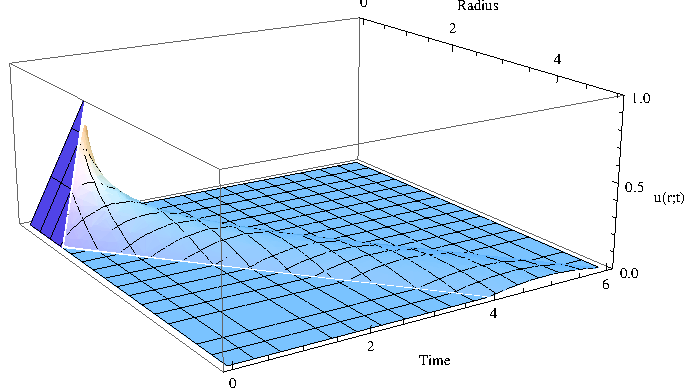
\includegraphics{13solution.pdf}
\label{13:solution}
\end{figure}

\appendix

\section{Derivation}\label{slproblem}
We will find the eigenvalues and eigenfunctions of the Sturm-Liouville eigenvalue problem 
\[\phi''(x) +\lambda \phi(x) = 0\]
for 
\[\phi(0)=0,\quad \phi'(L)=0.\]

We consider separately the case $\lambda=0$, $\lambda<0$, and $\lambda>0$.

In the case $\lambda=0$ the general solution to the problem is just 
\[\phi(x) = Ax+B\]
and applying boundary conditions we have 
\[ \phi(0) = A(0)+B=0 \]
\[\Rightarrow B = 0\]\\
and also
\[ \phi'(L) = A= 0\]
\[\Rightarrow A=0\]
So there are no nontrivial solutions to the Sturm-Liouville eigenvalue problem in this case.

In the case $\lambda=-\mu^2<0$ the general solution to the problem is just 
\[\phi(x)=Ae^{\mu x}+Be^{-\mu x}\]
and applying the boundary conditions we get 
\[\phi(0)=A+B=0\]
\[\Rightarrow-A=B\]
as well as 
\[\phi'(x)=A\mu e^{\mu x}-B \mu e^{-\mu x}\]
\[\phi'(L)=A\mu e^{\mu L}+A \mu e^{-\mu L}=0\]
but since $e^{\mu L} \neq -e^{-\mu L}$ for all $\mu L \in \mathbb{R}$ we must of necessity have
\[A=B=0.\]
Hence, there are no nontrivial solutions in this case either.

In the case $\lambda>0$ the general solution to the problem is just 
\[\phi(x) = A\cos{x\sqrt{\lambda}}+B \sin{x \sqrt{\lambda}}\]
applying boundary conditions we observe that
\[\phi(0) = A=0\]
and further that
\[\phi'(x) = B\sqrt{\lambda} \cos{x \sqrt{\lambda}}\]
\[\Rightarrow \phi'(L) = B\sqrt{\lambda} \cos{L \sqrt{\lambda}}=0\]
so all nontrivial solutions may be obtained by taking
\[B\neq 0 \quad  L\sqrt{\lambda}=\pi \left( \frac{1}{2} + n \right) \]

So taking the solutions in each of these cases together we see that all nontrivial solutions to the given Sturm-Liouville eigenvalue problem are of the form
\[ \lambda_n=\left( \frac{\pi}{L} \left( \frac{1}{2} + n \right) \right)^2  \quad \phi_n(x) =B \sin{x \sqrt{\lambda_n}} \quad n=1,2,\dots\]
for some arbitrary constant $B$.

\section{Check}\label{check}
We shall check that 
\[u=-\frac{1}{6} r^2\]
is a solution to
\[-1 = u_{rr} +\frac{2}{r} u_r \]

First we compute
\[u_r=-\frac{1}{3} r\]
and then
\[u_{rr}=-\frac{1}{3} \]

Now substituting we see that indeed 
\[ u_{rr} +\frac{2}{r} u_r = -\frac{1}{3} -\frac{2}{3} = -1 \]
as claimed.

\begin{thebibliography}{9}

	\bibitem{pinsky}
	  Mark Pinsky,
	  \emph{Partial Differential Equations and Boundary Value Problems with Applications}.
	  Waveland Press, Illinois,
	  3rd Edition,
	  2003.

	\bibitem{sc}
	  Wolfram MathWorld: Spherical Cap

	  \emph{http://mathworld.wolfram.com/SphericalCap.html}.

	\bibitem{si}
	  Wolfram MathWorld: Sphere Intersection

	  \emph{http://mathworld.wolfram.com/Sphere-SphereIntersection.html}.

	\bibitem{wikia}
	  Wikipedia: Spherical Cap

	  \emph{http://en.wikipedia.org/wiki/Spherical\_cap}.

	\bibitem{parseval}
	  Planet Math: Parseval's Equality

	  \emph{http://planetmath.org/encyclopedia/LyapunovEquation.html}.


\end{thebibliography}


\end{document}
